\section{\label{sec:nmp:example}Asynchronous System Example}
\newcommand*{\obinnod}[1]{Objects inside node 1 at the end of round #1}
\newcommand*{\obinrul}[2]{Objects inside node 1 after application of rule#1 during round #2}

This \namecref{sec:nmp:example} steps through a simple example of the evolution of \cref{sec:nmp:pespecific}'s asynchronous variant of \gls{nmp}.  The grid in question is found in \cref{fig:nmp:basicgrid}, and this example focuses on the node marked ``1''.  For simplicity, but without loss of generality, the example focuses on a border point in the grid, \ie{} a \gls{pe} with a \emph{three}-neighbourhood.  Two generations of \gls{nm} are shown (\ie{} the maximum generation count is 2: \(\cpfunc{i}{2}\)) for demonstration purposes.  Node 1 starts in state \(s_1\) and its adjacency list object is \(\cpfunc{a}{\cpfunc{n}{2} \; \cpfunc{n}{3} \;\cpfunc{n}{4}}\).

\begin{figure}
    \centering
    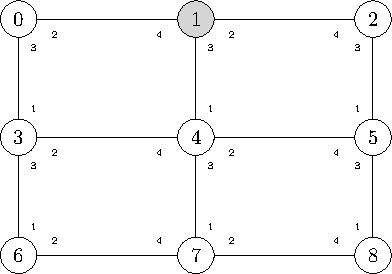
\includegraphics[keepaspectratio,width=0.7\textwidth,height=0.3\textheight]{chapters/nmp/images/3by3gridgraph.pdf}
    \caption[Basic 3×3 grid graph used for the example]{Basic 3×3 grid graph used for the example.  This example will focus on the perspective of node 1.  Other nodes are assumed to work equivalently, but their evolution is not discussed.  Nodes are labelled internally with their ID in the system (\(\iota\) in \cref{fig:nmp:iota_proxels_environment_oracle}), and each intermediary channel with the identity assigned to it by the nearby \gls{pe}.}
    \label{fig:nmp:basicgrid}
\end{figure}

\fxwarning{From José}{Embodying the unknown processes of the oracle, the data for the received \(v\) terms have been randomly generated for this example and have no particular significance.}

To supply a partial demonstration of the expected operation of the rule(s) which would replace the oracle, the contents of outgoing messages are computed according to the following simple rule: \cpruleinline{\cprule*{s_4}{\cprecv{\cpvw{W}{G}{\cpfunc{d}{A} \; \cpfunc{d}{B}}}{\iota}}{1}{s_5}{\cpsend{\cpvw{W}{G}{AB}}{\iota}}}  This rule merely sums the data received, and returns the newly computed outgoing message to the relevant node.

\setcounter{traces}{-1}

The total trace for this example is: \tracn{{\label{trace:0}}--}{--}{--} \tarr{} \tracn{\label{trace:1}0?*}{0?*}{0?*} \tarr{} \tracn{\label{trace:2}1?*}{0}{1?} \tarr{} \tracn{\label{trace:3}1}{0}{2?} \tarr{} \tracn{\label{trace:4}2?}{1?**}{2} \tarr{} \tracn{\label{trace:5}2}{2?}{2} \tarr{} \tracn{\label{trace:6}--}{--}{--}.  The state of Node 1 at the end of each round is shown in \crefrange{objs:nmp:ex0}{objs:nmp:ex6}.  Where the contents of a complex term change between the end of one round and the end of the next, the term and its changed contents are set in boldface to highlight the modifications.

\begin{cpobjectsfloat}
\begin{cpobjects}
\cpobjectsline{\cpfunc{a}{\cpfunc{n}{2} \, \cpfunc{n}{3} \, \cpfunc{n}{4}}}
\end{cpobjects}
\caption{\label{objs:nmp:ex0}Objects present inside Node 1 at the end of round 0 in the asynchronous \gls{nmp} example}
\end{cpobjectsfloat}

\paragraph{Round One}
This round is where node 1 receives its inputs from the environment by rules \cpruleref*{rule:nmp:proxspec:initcounter} and \cpruleref*{rule:nmp:proxspec:recvinputs}.  The maximum message generations counter, and the messages with the initial data for the \gls{pe} come through the channel connected to the environment.  Node 1 starts this round holding only its adjacency list, in this case \(\cpfunc{a}{\cpfunc{n}{2} \, \cpfunc{n}{3} \, \cpfunc{n}{4}}\).

The receipt of messages for all three neighbours causes \cpruleref{rule:nmp:proxspec:makews} to apply and node 1 to enter the sending cycle.  Two new \gls{oq} \(w\) messages are generated relating to each neighbour (because the other two neighbours will take the place of \(Y\) in applications of \cpruleref{rule:nmp:proxspec:makews}a --- recall that there is no \(Z\) in the rule for this node, as it only has three neighbours).  \cpRuleref{rule:nmp:proxspec:uniq} eliminates these duplicates, however, leaving one copy of each message for \cpruleref{rule:nmp:proxspec:sendtooracle} to send to the oracle.  These outgoing messages to the oracle are \(\cpvw{2}{1}{\cpfunc{d}{4} \, \cpfunc{d}{7}}\), \(\cpvw{3}{1}{\cpfunc{d}{1} \, \cpfunc{d}{7}}\) and \(\cpvw{4}{1}{\cpfunc{d}{1} \, \cpfunc{d}{4}}\) for neighbours 2, 3, and 4, respectively.

Node 1 then enters a `blocking wait' (see \cref{sec:cps:blocking}) and remains inactive until the oracle returns the new \gls{nm} messages to send to each neighbour.  \cpRuleref{rule:nmp:proxspec:recvfromoracle} sees node 1 receive those messages and then immediately forward them to the neighbours.  The messages are not stored inside node 1 at the end of a step.  Following the example oracle rule described above, the messages sent from the oracle to node 1 are \(\cpvv{2}{1}{11}\), \(\cpvv{3}{1}{8}\) and \(\cpvv{4}{1}{5}\) for neighbours 2, 3, and 4, respectively.

The application of \cpruleref{rule:nmp:proxspec:recvfromoracle} brings the sending cycle to a close, and node 1 moves to state \(s_5\).  In this state, \cpruleref{rule:nmp:proxspec:clearrs} clears away any receipt tokens present in the \gls{pe} then node 1 moves to the termination check of \cpruleref{rule:nmp:proxspec:movetoend}.  At this point, none of the \(v\) messages hold generation counters equal to the maximum generation count, and so processing will continue.  Finally, node 1 proceeds with another blocking wait, until messages arrive from any of its neighbours.

\begin{cpobjectsfloat}
\begin{cpobjects}
\cpobjectsline{\cpfunc{a}{\cpfunc{n}{2} \, \cpfunc{n}{3} \, \cpfunc{n}{4}} \quad \cpfunc{\mathbf{i}}{\mathbf{2}} \quad \cpvvbf{\mathbf{2}}{\mathbf{0}}{\mathbf{1}} \; \cpvvbf{\mathbf{3}}{\mathbf{0}}{\mathbf{4}} \; \cpvvbf{\mathbf{4}}{\mathbf{0}}{\mathbf{7}}}
\end{cpobjects}
\caption{\label{objs:nmp:ex1}Objects present inside Node 1 at the end of round 1 in the asynchronous \gls{nmp} example}
\end{cpobjectsfloat}

\paragraph{Round Two}
The second round proceeds similarly to the first, but with two key differences.  Firstly, the incoming messages are received from neighbouring \glspl{pe} via the channels connecting node 1 to them.  Secondly, messages are received only from neighbours 2 and 4.  This generates receipt tokens for those neighbours and sees node 1 enter a new sending cycle.

The presence of receipt tokens for both neighbours 2 and 4 leads to the creation of two duplicate \(w\) \gls{oq} messages about neighbour 3.  In effect, 1 and 3 swap roles as \(X\) and \(Y\) in \cpruleref{rule:nmp:proxspec:makews}.  Again, \cpruleref{rule:nmp:proxspec:uniq} eliminates the duplicate, and the single message \(\cpvw{3}{2}{\cpfunc{d}{9} \, \cpfunc{d}{5}}\) is sent to the oracle by \cpruleref{rule:nmp:proxspec:sendtooracle}.  In turn, by \cpruleref{rule:nmp:proxspec:recvfromoracle}, node 1 receives back \(\cpvv{3}{2}{14}\) and forwards it to neighbour 3, completing the sending cycle.  This is also the final message sent to neighbour 3, given that the maximum generation count for this system is two.

As before, node 1 moves from sending to clearing receipt tokens, checking whether it has completed \gls{nm}, and finally becomes quiescent once more, awaiting further messages from neighbours.

\begin{cpobjectsfloat}
\begin{cpobjects}
\cpobjectsline{\cpfunc{a}{\cpfunc{n}{2} \, \cpfunc{n}{3} \, \cpfunc{n}{4}} \quad \cpfunc{i}{2} \quad \cpvvbf{2}{\mathbf{1}}{\mathbf{9}} \; \cpvv{3}{0}{4} \; \cpvvbf{4}{\mathbf{1}}{\mathbf{5}}}
\end{cpobjects}
\caption{\label{objs:nmp:ex2}Objects present inside Node 1 at the end of round 2 in the asynchronous \gls{nmp} example}
\end{cpobjectsfloat}

\paragraph{Round Three}
Round three begins with receiving a single message, the final message to be received from neighbour 4.  Unlike the earlier rounds, no new messages are sent out due to said receipt.  Neighbour 4 was already one of the neighbours with the highest generation count among the messages stored in node 1, and so while it can serve as \(X\) in \cpruleref{rule:nmp:proxspec:makews}, neither of neighbours 2 or 3 can serve as \(Y\) because their generation counts are lower than neighbour 4's.

The fact that \cpruleref{rule:nmp:proxspec:makews} does \emph{not} apply means that \cpruleref{rule:nmp:proxspec:skiptorecv} \emph{is} applied --- for the first time in this system's evolution.  \cpRuleref{rule:nmp:proxspec:skiptorecv} unconditionally transitions node 1 back to removing all extant receipt tokens, before progressing to the termination check and then returning to awaiting new messages.

\begin{cpobjectsfloat}
\begin{cpobjects}
\cpobjectsline{\cpfunc{a}{\cpfunc{n}{2} \, \cpfunc{n}{3} \, \cpfunc{n}{4}} \quad \cpfunc{i}{2} \quad \cpvv{2}{1}{9} \; \cpvv{3}{0}{4} \; \cpvvbf{4}{\mathbf{2}}{\mathbf{2}}}
\end{cpobjects}
\caption{\label{objs:nmp:ex3}Objects present inside Node 1 at the end of round 3 in the asynchronous \gls{nmp} example}
\end{cpobjectsfloat}

\paragraph{Round Four}
This time, neighbour 2 sends its final message, and neighbour 3, at last, sends its first message.  The receipt from neighbour 3 leads to two new single instances of messages relating to neighbours 2 and 4.  The receipt from neighbour 2 could ordinarily lead to another message to be sent to neighbour 3, as it would pair up with neighbour 4 to act as \(X\) and \(Y\), respectively, in \cpruleref{rule:nmp:proxspec:makews}.  This does not occur, however, as neighbour 2 (and 3) has reached the maximum generation count, so \cpruleref{rule:nmp:proxspec:makews} is no longer applicable for it.

The messages to go to the oracle due to the receipt from neighbour 3 are \(\cpvw{2}{2}{\cpfunc{d}{3} \, \cpfunc{d}{2}}\) and \(\cpvw{4}{2}{\cpfunc{d}{8} \, \cpfunc{d}{3}}\).  Thus, the messages returned by the oracle and sent to neighbour 2 and are \(\cpvv{2}{2}{5}\) and \(\cpvv{4}{2}{11}\).  These are the last two messages to be sent by node 1 to its neighbours.

\begin{cpobjectsfloat}
\begin{cpobjects}
\cpobjectsline{\cpfunc{a}{\cpfunc{n}{2} \, \cpfunc{n}{3} \, \cpfunc{n}{4}} \quad \cpfunc{i}{2} \quad \cpvvbf{2}{\mathbf{2}}{\mathbf{8}} \; \cpvvbf{3}{\mathbf{1}}{\mathbf{3}} \; \cpvv{4}{2}{2}}
\end{cpobjects}
\caption{\label{objs:nmp:ex4}Objects present inside Node 1 at the end of round 4 in the asynchronous \gls{nmp} example}
\end{cpobjectsfloat}

\paragraph{Round Five}
Only one more message is still to be received, from neighbour 3 specifically. Node 1 will wait until said message is received, but at that point, all message generation counters will be equal to the maximum, and thus no further messages will be sent to its neighbours.

Following the application of \cpruleref{rule:nmp:proxspec:recvfromneighs} to receive the final message from neighbour 3, node 1 returns to state \(s_2\) and the rules are again explored in top-down order.  This time, \cpruleref{rule:nmp:proxspec:makews} is inapplicable, so \cpruleref{rule:nmp:proxspec:skiptorecv} is applied, transitioning node 1 to state \(s_5\).  \cpRuleref{rule:nmp:proxspec:skiptorecv} is the only rule applied at this step because it is the only rule which moves from state \(s_2\) to state \(s_5\).  Next, \cpruleref{rule:nmp:proxspec:clearrs} deletes the last receipt token.  Again, \cpruleref{rule:nmp:proxspec:clearrs} is the only rule applied because it is the only one to use that specific state transition.  Finally, without any \(v\) messages with a generation count below the maximum present in the \gls{pe}, node 1 moves to state \(s_7\) and the finalisation phase by \cpruleref{rule:nmp:proxspec:movetoend}.

\begin{cpobjectsfloat}
\begin{cpobjects}
\cpobjectsline{\cpfunc{a}{\cpfunc{n}{2} \, \cpfunc{n}{3} \, \cpfunc{n}{4}} \quad \cpfunc{i}{2} \quad \cpvv{2}{2}{8} \; \cpvvbf{3}{\mathbf{2}}{\mathbf{7}} \; \cpvv{4}{2}{2}}
\end{cpobjects}
\caption{\label{objs:nmp:ex5}Objects present inside Node 1 at the end of round 5 in the asynchronous \gls{nmp} example}
\end{cpobjectsfloat}

\paragraph{Round Six}
Round six is the final round of the evolution of the system, for node 1 at least.  With node 1 in state \(s_7\), the only applicable rule is \cpruleref{rule:nmp:proxspec:finaloracle}.  The effect of \cpruleref{rule:nmp:proxspec:finaloracle} is to send every \(v\) message stored in node 1 to the oracle, renaming them to \(w'\) messages so that the oracle recognises them as finalisation messages rather than \gls{oq} messages for \gls{nm} purposes.

Eventually, the oracle will return the final result message, with the contained datum computed by some means from the messages the oracle received from node 1.  That message is immediately forwarded back to the environment, and evolution of node 1 halts.  Once all other nodes have halted, evolution of the system will have terminated.

\begin{cpobjectsfloat}
\begin{cpobjects}
\cpobjectsline{\cpfunc{a}{\cpfunc{n}{2} \, \cpfunc{n}{3} \, \cpfunc{n}{4}} \quad \cpfunc{i}{2}}
\end{cpobjects}
\caption{\label{objs:nmp:ex6}Objects present inside Node 1 at the end of round 6 in the asynchronous \gls{nmp} example}
\end{cpobjectsfloat}